\chapter{文献综述}
\label{cha:china}

\section{本章引言}
域间路由作为互联网领域的重要问题,属于网络控制平面的功能,集中式的网络管理控制对解决域间路由提供了很重要的思路。本章节主要介绍域内路由协议及其工作原理、内部域内路由协议iBGP存在问题、现有解决iBGP可扩展问题的方案、集中式思路优化BGP的相关研究等内容。

\section{BGP协议及其工作流程}

网络中信息传输需要经过多台路由器进行转发,路由器上运行的路由协议会生成路由信息表,路由信息表记录了信息转发的下一跳地址,即应转发到哪台路由器。信息是否能准确从源地址发送到目的地址,路由协议至关重要。路由协议\cite{DianeTeare2016CCNP}可以使用内部或者外部分类为:内部网关协议(Interior Gateway Protocol, IGP)和外部网关协议(Exterior Gateway Protocol, EGP)。IGP协议负责在一个自治系统内交换路由信息,EGP协议负责在不同自制系统间交换传递路由信息。边界网关协议BGP\cite{rfc1771}属于EBGP协议的一种,是运行于传输控制协议(Transmission Control Protocol, TCP)上的一种自治系统的路由协议, 它的主要功能是和其他的BGP系统交换网络可达信息。运行在自治系统间的BGP协议称之为eBGP协议(External Border Gateway Protocol, eBGP)。运行在自治系统内部的BGP协议称之为iBGP协议。

\begin{figure}
  \centering
  % Requires \usepackage{graphicx}
  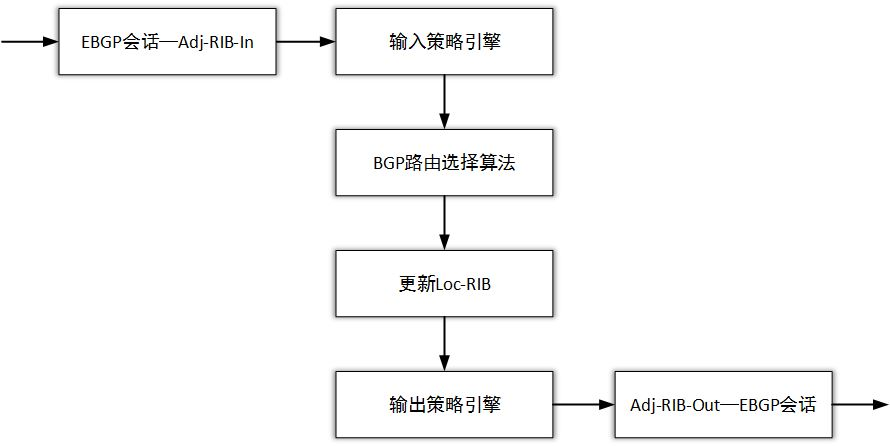
\includegraphics[width=\textwidth]{router}
  \caption{路由器的路由系统流程图}
  \label{fig:router}
\end{figure}

BGP协议运行在自治系统内的每台边界路由器上,每台边界路由器收到路由信息,会进行路由信息存储、应用路由策略、计算最优路由、更新本地路由表以及将路由进行出口过滤并转发等操作,其处理路由信息的流程如图\ref{fig:router}:所示,主要涉及三大模块:路由存储、路由策略、路由计算。

\subsection{路由存储}
运行BGP会话的边界路由器从其他对等体收到路由更新消息,其保留收到的信息,将信息进行处理生成最优路由用于本地数据包的转发,该边界路由器会基于预定义的策略向外宣告路由。在路由信息处理的过程中,路由信息存储在路由信息库(Routing Information Bases, RIBs)中,BGP的路由信息库\cite{rfc1771}中主要包含以下三张表:

\begin{itemize}
    \item Adj-RIBs-In:该表中存储了从不同对等体收到的未经路由入口过滤和属性修改的原始BGP路由信息,该信息用于BGP决策过程的输入。
    \item Local RIB:该表中存储了经过路由入口策略(过滤和BGP属性修改)的路由信息,此外该表中还使用selected标记了每一个前缀的最优路由。
    \item Adj-RIBs-Out:该表中存储了经过路由出口策略,即将被宣告给每一个对等体的最优路由信息。
  \end{itemize}

\subsection{路由策略}
路由信息在自治系统间传输,每个自治系统如何影响路由选择和传递,需要依赖该自治系统部署的路由策略\cite{DianeTeare2016CCNP},可以过滤更新从邻居收到的路由信息,经过路由计算之后也可以过滤更新将宣告给邻居的路由信息。

路有更新过滤包含四个部分:
\begin{itemize}
    \item 分布列表:通过配置访问列表对路由更新进行控制,配置路由器的网络管理员决定允许接收来自哪些IP的路由更新,拒绝接收哪些IP的路由更新。
    \item 前缀列表:针对从邻居收到或者转发给邻居的路由,应用前缀列表,对匹配上前缀列表正则表达式的前缀执行permit或者deny操作。
    \item AS-path访问列表:配置路由器的网络管理员根据eBGP路由中携带的AS-path属性内容,对路由信息进行过滤。
    \item route-map路由映射:路由映射在控制BGP更新方面非常灵活,可以匹配并设置多种不同的BGP属性。该操作分两部分:match匹配和set设置。如果路由匹配了一条route-map命令中的所有匹配项,说明该路由与之匹配,则执行路由映射命令中的设置(修改路由属性,permit或者deny)。
\end{itemize}


分布列表、前缀列表、AS-path访问列表、路由映射都可以用来入站出站路由的过滤更新,不同的路由设备中BGP过滤更新机制的执行顺序可能不同。本文研究实现基于Quagga\cite{quagga}软件路由器平台,Quagga的入站出站过滤更新顺序见下:

Quagga入站过滤更新顺序:分布列表、前缀列表、AS-path访问列表、路由映射。
Quagga出站过滤更新顺序:前缀列表、分布列表、AS-path访问列表、路由映射。

\subsection{路由选择算法}
BGP路由计算\cite{DianeTeare2016CCNP}的过程是为了选择最优路由,BGP最优路由的选择是根据BGP属性执行的。同一个前缀可能有多条路由,BGP会选择一条最优路由,来传输去往这个前缀目的地址的流量,不同的路由设备路由计算的算法有微小差异,以Quagga软件路由器中BGP的实现为例,同一条前缀的多跳路由(不构成AS环路且下一跳有效可达),根据收到时间由近及远,两两比较,得到最优路由。比较的过程如下所示,不断执行以下步骤直到选出最优路由:

\begin{itemize}
    \item 步骤1:优选权重(Weight)最高的路由,Weight属性本地路由器有效。
    \item 步骤2:优选本地优先级(Local Preference)最高的路由,自治系统内有效。
    \item 步骤3:优选本地路由器初始的路由(本地初始的路由在BGP表中的下一跳显示为0.0.0.0)。
    \item 步骤4:优选as-path最短的路由。
    \item 步骤5:优选源代码(Origin code)最小的路由(IGP<EGP<不完整路由)。
    \item 步骤6:优选MED最低的路径,只有当所有待选路由来自同一AS时,路由器才会对比MED。网络管理员也可以通过设置路由器配置命令bgp always-compare-med,使得MED值总是可比。
    \item 步骤7:优选外部eBGP路由,而不是内部iBGP路由。
    \item 步骤8:优选去往BGP下一跳最短的路径,即IGPcost最小的路由。
    \item 步骤9:优选eBGP最老的路由,减少路由反复启动和禁用的风险。
    \item 步骤10:优选邻居BGP路由器ID值router-id最低的路由。
    \item 步骤11:优选邻居IP地址最小的路由。
\end{itemize}

本小节介绍了BGP协议以其工作流程,熟悉BGP处理路由信息的流程有助于利用集中式的思路解决且优化iBGP存在的一些问题。

\section{iBGP协议存在的问题}

早期iBGP协议运行在某个自治系统内部的边界路由器上,因为iBGP连接中路由信息仅能传播一跳(域内的边界路由器收到iBGP邻居的路由信息,不能再将其进行转发传播),所以域内的iBGP路由器必须以全网状Full-mesh的结构相连,保证路由信息传输到每一台路由器,所以随着网络规模的不断扩大,自治系统内部的边界路由器逐渐增多,全网的路由越来越多(Potaroo显示先IPv4的路由表项约有70万条\cite{bgptabledata}),网络拓扑连接和路由策略越来越复杂,iBGP协议面临很大的挑战\cite{ibgp2016infocom},比如糟糕的可扩展性、配置文件的负担越来越大、域内用于路由信息传输的BGP控制报文占用更多的带宽资源、路由表的冗余存储等等。现在,传统的Full-mesh模式的iBGP结构仅应用于规模比较小的自治系统内,规模比较大的自治系统一般使用比较容易部署的路由反射器。

iBGP\cite{ibgp2016infocom}目前存在三方面问题:可扩展性差,域内路由决策非最优出口,复杂路由策略难以管理。
\begin{itemize}
\item iBGP协议必须保持全连接,防止在AS内部形成BGP路由环路,同时确保BGP路由路径上的所有路由器将数据报正确地转发到目的地。全连接导致每台边界路由器需要和域内的其他边界路由器维护iBGP会话,整个域内的iBGP会话数量是路由器的平方数量级,同时随着BGP路由表加速增长对路由器的存储和计算能力提出了更高的要求,iBGP的可扩展性问题日益显著。
\item 自治系统内的边界路由器收到路由后,会通过iBGP连接传播一条给相连的iBGP对等体。如果RR结构,路由反射器收到路由,会计算最优路由,将最优路由宣告给其他路由器,可能导致某些路由器没有收到全部路由。在路由计算的过程中,如果没有基于全部路由计算,或者仅考虑了IGP cost,没有考虑域内的拓扑等其他信息,这些均有可能导致自治系统内的iBGP路由计算结果非最优出口。
\item 自治系统的策略需要在自治系统内的每台边界路由器上进行配置,容易误配置,或者出现路由器策略配置不一致的现象。自治系统内复杂的路由策略分布在每台路由器上,难以管理。

\section{现有解决iBGP可扩展问题的相关研究}
本课题从解决iBGP的可扩展问题为切入点,调研现有解决iBGP可扩展问题的相关研究,其根据体系结构思想和设计,大致可以分成两类:分布式体系结构下的相关研究(路由反射、AS联邦)和集中式体系结构下的相关研究(SoftRouter、RCP、RFCP)。

\subsection{分布式体系结构下的相关研究}
传统的分布式体系结构:路由反射和AS联邦,解决了iBGP全连接引起的可扩展问题,但其设计本身可能导致选择路由不是最优出口、路由震荡、转发环路等问题。

\subsubsection{路由反射}
路由反射(图1)将自治系统内的边界路由器分成cluster。每个cluster里面有一个或者多个路由反射器,cluster中其他的路由器称之为client。Client仅与自己的RR建立iBGP连接,路由反射器之间全连接,宣告最优路由。RR收到路由并选择最优路由:如果该路由从非client的iBGP对等体收到,RR将最优路由反射给所有的clients;如果该路由从client的iBGP对等体收到,RR将最优路由反射给其他的RR和所在cluster里面的clients。Client只和自己的RR建立iBGP连接。

路由反射因为缺少全部路由和结构设计等问题,在特定条件下会产生非最优出口、转发环路、路由震荡等问题。

路由反射导致的非最优出口(图2),RR收到前缀Pre1,经过路由计算后发现C1为Pre1的最优出口,RR会将Pre1的最优出口为C1这条消息宣告给C2和C3,C3会认为Pre1的最优出口为C1,实际上对于C3而言,C2为Pre1的最优出口。

路由反射导致的转发环路(图3),C1和C2收到相同前缀Pre1;分别通告给自己的反射器,RR1认为Pre1的最优出口为C1;RR2认为Pre1的最优出口为C2。RR1收到目的地址为Pre1的包,判断该数据包的最优出口为C1,根据IGP将数据包转发给RR2。RR2收到目的地址为Pre1的包,判断该数据包的最优出口为C2,根据IGP转发给RR1。RR1又转发给RR2,RR2转发给RR1,形成转发环路。该种情况的根本原因为物理链路和逻辑链路不一致,路由反射器的最优出口的ospf路径经过其他的路由反射器。

\section{集中式思路优化BGP的相关研究}

路由反射导致的路由震荡有两种典型的情况:MED震荡和拓扑震荡。
路由反射导致的MED震荡(图4),根本原因在于路由计算的过程中某些度量值(MED)不可比。相同颜色的路由器为同一个cluster,RR1收到C1-1和C1-2的路由,选择来自C1-2[IGP小]的路由;RR2收到C1-2和C2的路由,选择来自C2[MED小]的路由;RR1收到C1-1、C1-2、C2(RR2向RR1宣告)的路由,先淘汰来自C1-2[MED大]的路由,最终选择来自C1-1[IGP小]的路由;RR2收到C1-1(RR1向RR2宣告)、C2的路由,选择C1-1[IGP小],产生了路由震荡。
路由反射导致的拓扑震荡(图5),相同颜色的路由器为同一个cluster,RR1收到来自C1的路由,选择来自C1的路由;RR2收到RR1宣告出来的来自C1的路由和来自C2的路由,根据IGP cost等度量,选择来自C2的路由;RR3收到RR1宣告出来的来自C1的路由、RR2宣告出来的来自C2的路由、来自C3的路由,选择RR1向外宣告的来自C1的路由;RR1收到来自C1和C2,选择C2(震荡)。该种情况产生的根本原因是RR结构设计不合理,cluster内部的RR和client的IGP cost远大于RR和其他cluster内的client,路由决策主要依赖IGP信息。
\subsubsection{AS联邦}
AS联邦(图6)的基本思想是将自治系统划分成多个子自治系统,子自治系统之间运行扩展的eBGP协议,子自治系统内部全连接,运行iBGP协议。

AS联邦因为缺少全部路由和MED度量值不可比等问题,在特定条件下会产生非最优出口、路由震荡等问题。
AS联邦导致的非最优出口(图7),Ra收到来自Rb和Rc的路由Pre,Ra根据IGP cost选择来自Rc的路由Pre,Rd收到Ra宣告的来自Rc的路由,Rd认为Pre的最优出口为Rc,实际上Rd的最优出口是Rb。

AS联邦导致的MED路由震荡(图8),Ra选Rb(MED去除Rc, IGP去除Re), Rd选Rb(IGP), Ra选Rc(IGP), Rd选Re(MED), Ra选Rb(路由发生Loop)。

\subsection{集中式体系结构下的相关研究}
新型的集中式体系结构:SoftRouter、RCP、RFCP,解决了iBGP的可扩展问题,对路由存储、路由计算、策略优化某个方面进行了优化。
\subsubsection{SoftRouter}
SoftRouter(图9)的基本思想是将主控板(控制平面)从传统路由器中分离,配有主控板的路由器作为控制单元,配有线卡的路由器作为转发单元,转发单元和控制单元多对多动态绑定,转发单元通过ForCES协议获得控制单元的转发表。

SoftRouter解决了iBGP可扩展问题。FE可以动态绑定到多个CE上,不同CE执行路由器不同的功能,则SoftRouter容易开发新功能。此外,主控板减少,运营商的开支也相对应地减少。Softrouter也存在一定的局限性,因为CE和FE多对多,所以Softrouter结构复杂,本身可扩展性较差;在路由计算的过程中,仍使用传统的主控板进行计算,没有考虑IGP视图;FE不同的功能策略在不同的CE上进行配置,不同CE策略可能存在矛盾、覆盖等情况。

\subsubsection{RCP}
RCP(Route Control Platform,图10)是在自治系统内部建立一个集中控制平台,通过与AS内边界路由器建立iBGP连接来接收路由。在RCP平台上进行集中式路由计算和策略管理,如果邻居AS也部署了RCP平台,那么RCP平台之间可以直接建立BGP连接进行通信,这种方式有助于域间新协议的发展。

RCP可以集中式路由存储;集中式策略配置,方便网络操作员配置;有集中计算资源、IGP拓扑和全部路由进行路由计算。但是因为RCP平台本身支持iBGP、eBGP连接,平台可扩展性较差;在策略集中配置的过程中未考虑对集中的策略配置进行检测,预防策略冲突、覆盖等问题。RCP的路由计算仍属于传统的分布式路由计算,计算N次得到N台路由器的最优出口路由。

\subsubsection{RFCP}
RFCP(Route Flow Control Platform,图11)是基于SDN的思想,集中式地收集信息,在APP运行多台虚拟机,模拟自治系统环境,分布式地计算路由,并通过SDN平台传递给真实自治系统内的边界路由器。

RFCP可以集中式地对数据进行管理,通过流表规则下发对数据包和路由信息包进行转发,但RFCP结构中路由表冗余存储、路由计算未考虑IGP拓扑且仍为分布式计算,路由策略通过南向接口将策略传给控制器,未集中配置。

\section{本章小结}

综合以上的调研,RR、AS联邦、3种集中式体系结构的方案虽然解决了iBGP可扩展问题,但RR和AS联邦带来了新问题;3种集中式方案对路由存储、计算、策略管理的某些方面进行优化,具体的对比见图13。
本课题提出新结构,能够解决iBGP可扩展性,同时最大限度优化路由存储和计算、策略管理。路由表RIB仅存储在集中控制平台,路由计算在集中平台上计算,依赖自治系统内的网络拓扑信息,支持多输入多输出的计算模式,拟计算一次(最坏情况下计算N次)得出所有边界路由器针对Prefix的最优路由。
